%!TeX root=../tese.tex
%("dica" para o editor de texto: este arquivo é parte de um documento maior)
% para saber mais: https://tex.stackexchange.com/q/78101/183146

%% ------------------------------------------------------------------------- %%
\chapter{Problema Estático}
\label{cap:problema-estatico}

Neste capítulo será apresentado a solução para encontrar uma árvore binária de busca estática com custo mínimo para uma determinada entrada. O algoritmo foi desenvolvido por \cite{knuth}.

\section{Cálculo do custo}

O custo de um acesso à chave $x_i$ em uma ABB estática é o número de nós acessados durante o algoritmo de busca. Como rotações não são permitidas em ABBs estáticas, a estrutura da árvore não muda, logo o custo de um acesso à chave $x_i$ nesta ABB sempre é a profundidade de $x_i$ + 1. Denotaremos a profundidade do nó $x_i$ como $d(x_i)$.

O custo para uma ABB estática executar uma sequência $X = (x_{1},\ldots,x_{m})$ de $m$ acessos às chaves $x_{1}, x_{2},\ldots,x_{n}$ é a somatória dos custos dos acessos executados. 

\begin{align*}
    custo = \sum_{i=1}^{m} d(x_i) + 1
\end{align*}

Uma delimitação óbvia para este custo é que ele é no mínimo $m$, uma vez que haverá $m$ acessos e o custo mínimo para cada acesso é $1$.

%Um algoritmo é chamada de \textit{offline} se tem conhecimento da sequência $X$ antes de começar os acessos as chaves de $X$. Neste contexto, é possível desenvolver algoritmos para inicializar a ABB da maneira mais eficiente levando em conta que sabemos a sequência de chaves a serem acessadas.

Dada uma sequência $X$ de acessos, uma ABB é considerada ótima se executa os acessos de $X$ com o menor custo possível.

\section{Natureza do problema}

Denotaremos por $e(x_i)$ o número de ocorrências de $x_i$ em X.

Definimos o custo total de uma sequência de buscas com base em cada elemento de $X$. Porém, nota-se que é possível definir o mesmo custo com base no número de ocorrências de cada elemento da ABB. Cada acesso ao nó $x_j$ contribui com $d(x_j) + 1$ ao custo, como $x_j$ será acessado $e(x_i)$ vezes, então o nó $x_j$ contribui com $(d(x_j) + 1)  \cdot e(x_j)$ para o custo total.

\begin{align*}
\sum_{i=1}^{m} d(x_i) + 1 &= \sum_{j=1}^{n} (d(x_j) + 1) \cdot e(x_j)
\end{align*}


Dado que a contribuição de um nó para o custo é uma multiplicação entre a sua profundidade e seu número de ocorrências, intuitivamente é esperado que os nós mais próximos da raiz da ABB ótima sejam os nós com os maiores números de ocorrência, já que a ABB terá que acessar esse nó múltiplas vezes. Analogamente, é esperado que os nós mais distantes da raiz da ABB ótima sejam os nós com os menores números de ocorrência.

De maneira sucinta, é esperado que o custo de acessos mais caros, ou seja, acessos a nós mais profundos, sejam pagos menos vezes e é esperado que os custos de nós mais baratos, ou seja, acessos a nós mais superficiais, sejam pagos mais vezes.

\section{Algoritmo Guloso}

É possível desenvolver um algoritmo guloso para a construção da ABB com base nessa intuição de priorizar que nós com maior número de ocorrência estejam mais próximos da raiz. O Programa~\ref{prog:abb-gulosa}: organiza os nós de maneira decrescente no número de ocorrências e adiciona iterativamente à árvore o nó com maior número de ocorrências que ainda não foi adicionado.

\begin{programruledcaption}{Algoritmo guloso ABB.\label{prog:abb-gulosa}}
  \begin{lstlisting}[
    language={[brazilian]pseudocode},
    style=pseudocode,
    style=wider,
    functions={},
    specialidentifiers={},
  ]
      funcao guloso_ABB(chaves, ocorrências)
        fila_prioridade := fila_de_prioridade() // Declaração de uma fila de   prioridade vazia
        abb := abb() // Declaração de uma ABB vazia
        para i de 1 até chaves.tamanho() faça
            fila_prioridade.insere({chaves[i], occorências[i]}) // Fila de prioridade está ordenando de maneira decrescente no segundo parâmetro
        enquanto prioridade_mínima.tamanho() != 0 // Há nós para serem adicionados
            novo_nó := prioridade_mínima.remove()
            abb.insere(novo_nó)
	  devolva abb
  \end{lstlisting}
\end{programruledcaption}

Apesar da abordagem acima ser bastante promissora, priorizar unicamente o número de ocorrências não garante adquirir a solução ótima. Isso acontece porque a posição de cada nó na árvore influencia a profundidade mínima de todos os nós abaixo, principalmente levando em conta a propriedade de árvores binárias que todos os nós filhos esquerdos são menores que os pais e todos os nós filhos direitos são maiores. Assim, em algumas situações, é mais vantajoso ter como pai um nó com menor número de ocorrências e chave intermediária e ter nós com maior número de ocorrências mais profundos. Isto se torna ainda mais evidente quando pensamos em entradas com número de ocorrências por nó muito parecidos, nestes casos a estrutura de uma árvore binária mais balanceada tende a ser melhor.


\begin{figure}[h]
\centering
\begin{minipage}[c]{0.3\textwidth}
\centering
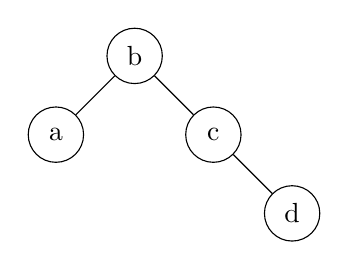
\begin{tikzpicture}
  [node/.style={circle,draw,minimum size=2em}]
  \node[node] (A) at (-1,-1) {a};
  \node[node] (B) at (0,0) {b};
  \node[node] (C) at (1,-1) {c};
  \node[node] (D) at (2,-2) {d};
  
  \draw (A) -- (B);
  \draw (B) -- (C);
  \draw (C) -- (D);
\end{tikzpicture}
\end{minipage}
\begin{minipage}[c]{0.3\textwidth}
\centering
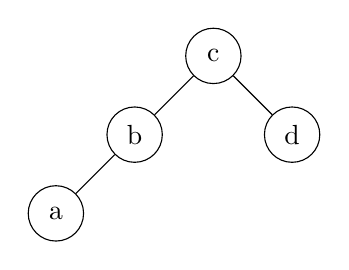
\begin{tikzpicture}
  [node/.style={circle,draw,minimum size=2em}]
  \node[node] (A) at (-2,-2) {a};
  \node[node] (B) at (-1,-1) {b};
  \node[node] (C) at (0,0) {c};
  \node[node] (D) at (1,-1) {d};
  
  \draw (A) -- (B);
  \draw (B) -- (C);
  \draw (C) -- (D);
\end{tikzpicture}
\end{minipage}
\begin{minipage}[c]{0.3\textwidth}
\centering
\begin{tabular}{|c|c|}
\hline
\multicolumn{2}{|c|}{\textbf{Número de ocorrências}} \\
\hline
\textbf{$a$} & 5 \\
$b$ & 15 \\
$c$ & 10 \\
$d$ & 10 \\
\hline
\end{tabular}
\end{minipage}
\caption{Respectivamente: Árvore gerada pelo algoritmo guloso com custo total 75. Árvore ótima com custo total 65. Tabela do número de ocorrências por chave na sequência de entrada.}
\end{figure}

\section{Algoritmo Ótimo}

A análise acima nos leva a perceber que precisamos de uma conduta que considere tanto o número de ocorrências de cada nó quanto a estrutura da árvore em si.

O algoritmo ótimo foi desenvolvido por \cite{knuth}.

Primeiramente é preciso entender como a estrutura da árvore ótima está disposta. Consideremos que a árvore possui as chaves em um intervalo contínuo de 1 até $n$. 

Para uma árvore $T$ com chave $k$ como raiz ser ótima, então a raiz possui uma sub-árvore ótima contendo as chaves $1,\dots,k$ como filha esquerda e outra sub-árvore ótima contendo as chaves $k$+1$,\dots,n$ como filha direita.

Isso pode ser provado da seguinte maneira: Seja $T$ uma árvore ótima para uma entrada $X$ com chave $k$ na raiz e seja $T'$ a sub-árvore de $k$ que não é ótima. Como $T'$ não é ótima, então existe uma árvore $T''$ ótima que também possui as mesmas chaves de $T'$, mas possui custo menor para os acessos de $X$. Assim, é possível trocar a sub-árvore $T'$ pela sub-árvore $T''$ em $T$ e encontramos uma árvore com custo menor que $T$. Como $T$ é uma árvore ótima, isso é uma contradição.

Assim, sabemos que para um intervalo $k_i, \ldots, k_j$ ($i \leq j$), a árvore ótima possui um nó com chave $k_r$ ($i \leq r \leq j$) como raiz e duas subárvores possivelmente vazias como filhas. A sub-árvore esquerda é uma árvore ótima que contém as chaves $k_i, \ldots, k_{r-1}$ e a sub-árvore direita é uma árvore ótima que contém as chaves $k_{r+1}, \ldots, k_j$.

Levando em consideração essa estrutura, dado um intervalo de chaves $k_i, \ldots, k_j$, o algoritmo ótimo precisa descobrir qual das chaves deve se tornar o nó raiz para minimizar o custo total.